\documentclass[a4paper,11pt]{report}
\usepackage[showexo=true,showcorr=false]{../packages/coursclasse}

% - Simplification et amplification de fractions
% - Fractions irréductibles
% - Ecriture décimale à fraction irréductible
% - Fractions équivalentes
% - Comparaison de fractions

%Commenter ou enlever le commentaire sur la ligne suivante pour montrer le niveau
\toggletrue{montrerNiveaux}
%permet de gérer l'espacement entre les items des env enumerate et enumitem
\usepackage{enumitem}
\setlist[enumerate]{align=left,leftmargin=1cm,itemsep=10pt,parsep=0pt,topsep=0pt,rightmargin=0.5cm}
\setlist[itemize]{align=left,labelsep=1em,leftmargin=*,itemsep=0pt,parsep=0pt,topsep=0pt,rightmargin=0cm}
%permet de gerer l'espacement entre les colonnes de multicols
\setlength\columnsep{20pt}

   

\begin{document}
%%%%%%%%%%%%%%%%% À MODIFIER POUR CHAQUE SERIE %%%%%%%%%%%%%%%%%%%%%%%%%%%%%
\newcommand{\chapterName}{Espace}
\newcommand{\serieName}{Représentation de solides}


%%%%%%%%%%%%%%%%%% PREMIERE PAGE NE PAS MODIFER %%%%%%%%%%%%%%%%%%%%%%%%
% le chapitre en cours, ne pas changer au cours d'une série
\chapter*{\chapterName}
\thispagestyle{empty}

%%%%% LISTE AIDE MEMOIRE %%%%%%
\begin{amL}{\serieName}{
\item Représentation d’un objet dans l’espace (page 142)
\item Prisme droit (page 145)
\item Parallélépipède rectangle ou pavé droit (page 146)
}
\end{amL}
%%%%%%%%%%%%%%% DEBUT DE LA SERIE NE PAS MODIFIER %%%%%%%%%%%%%%%%%%%%%%%%%%%%%
\section*{\serieName}
\setcounter{page}{1}
\thispagestyle{firstPage}



%%%%%%%%%%% LES EXERCICES %%%%%%%%%%%%%%%%%%%%%%%%%%%%%%%%%%%
\begin{exof}{ES97}{143}{1}
\end{exof}
\begin{exof}{ES98}{144}{1}
\end{exof}
\begin{exol}{ES99}{118}{1}
\end{exol}
\begin{exol}{ES100}{118}{3}
\end{exol}
\begin{exop}{
Parmi les représentations suivantes, lesquelles sont des représentation en perspective cavalière?	
Justifie.
\begin{tasks}(3)
		\task 

		\begin{tikzpicture}
% front face
\coordinate (A) at (-1,0);
\coordinate (B) at (0,2);
\coordinate (C) at (1,0);
% vector v defines the leakage angle
\coordinate (v) at (.8,.8);
\coordinate (w) at (.5,.5);
\draw (A)--(B)--(C)--cycle;
% back face
\coordinate (A') at ($(A)+(v)$);
\coordinate (B') at ($(B)+(v)$);
\coordinate (C') at ($(C)+(w)$);
\draw[dashed] (C')--(A')--(B');
\draw (B')--(C');
\draw[dashed](A)--(A');
\draw(B)--(B');
\draw(C)--(C');
\end{tikzpicture}

		\task 

		\begin{tikzpicture}
% front face
\coordinate (A) at (-1,0);
\coordinate (B) at (0,2);
\coordinate (C) at (1,0);
% vector v defines the leakage angle
\coordinate (v) at (.8,.8);
\draw (A)--(B)--(C)--cycle;
% back face
\coordinate (A') at ($(A)+(v)$);
\coordinate (B') at ($(B)+(v)$);
\coordinate (C') at ($(C)+(v)$);
\draw[dashed] (C')--(A')--(B');
\draw (B')--(C');
\draw[dashed](A)--(A');
\draw(B)--(B');
\draw(C)--(C');
\end{tikzpicture}

		\task 

		\begin{tikzpicture}
% front face
\coordinate (A) at (-1,0);
\coordinate (B) at (0,2);
\coordinate (C) at (1,0);
% vector v defines the leakage angle
\coordinate (w) at (.8,.8);
\coordinate (w) at (.5,.5);
\draw (A)--(B)--(C)--cycle;
% back face
\coordinate (A') at ($(A)+(w)$);
\coordinate (B') at ($(B)+(w)$);
\coordinate (C') at ($(C)+(w)$);
\draw (C')--(A')--(B');
\draw (B')--(C');
\draw(A)--(A');
\draw(B)--(B');
\draw(C)--(C');
\end{tikzpicture}
\task

	\begin{tikzpicture}
\rotateRPY{0}{55}{0}
\begin{scope}[RPY]
% front face
\coordinate (A) at (-2,0);
\coordinate (B) at (0,2);
\coordinate (C) at (1,0);
% vector v defines the leakage angle
\coordinate (v) at (.7,.7);
\draw (A)--(B)--(C)--cycle;
% back face
\coordinate (A') at ($(A)+(v)$);
\coordinate (B') at ($(B)+(v)$);
\coordinate (C') at ($(C)+(v)$);
\draw[dashed] (C')--(A')--(B');
\draw (B')--(C');
\draw[dashed](A)--(A');
\draw(B)--(B');
\draw(C)--(C');
\end{scope}
\end{tikzpicture}
\task

\begin{tikzpicture}
\rotateRPY{0}{55}{0}
\begin{scope}[RPY]
% front face
\coordinate (A) at (-1,0);
\coordinate (B) at (0,2);
\coordinate (C) at (1,0);
% vector v defines the leakage angle
\coordinate (v) at (.7,.7);
\draw (A)--(B)--(C)--cycle;
% back face
\coordinate (A') at ($(A)+(v)$);
\coordinate (B') at ($(B)+(v)$);
\coordinate (C') at ($(C)+(v)$);
\draw (C')--(A')--(B');
\draw (B')--(C');
\draw (A)--(A');
\draw (B)--(B');
\draw (C)--(C');
\end{scope}
\end{tikzpicture}
		\task

		\begin{tikzpicture}

\rotateRPY{10}{80}{0}
\begin{scope}[RPY]
% front face
\coordinate (A) at (-1,0);
\coordinate (B) at (0,2);
\coordinate (C) at (1,0);
% vector v defines the leakage angle
\coordinate (v) at (.8,.8);
\coordinate (w) at (.5,.5);
\draw (A)--(B)--(C)--cycle;
% back face
\coordinate (A') at ($(A)+(v)$);
\coordinate (B') at ($(B)+(v)$);
\coordinate (C') at ($(C)+(v)$);
\draw[dashed] (C')--(A')--(B');
\draw (B')--(C');
\draw[dashed](A)--(A');
\draw(B)--(B');
\draw(C)--(C');
\end{scope}
\end{tikzpicture}
\end{tasks}
	}{1}
\end{exop}

\newpage
\begin{exop}{
Parmi les représentations suivantes, lesquelles sont des représentation en perspective cavalière?	
Justifie.

\begin{tasks}(3)
	\task 

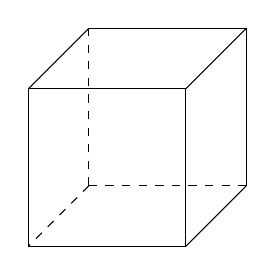
\begin{tikzpicture}
   \coordinate (a) at (-1,-1,-1);
    \coordinate (b) at (-1,-1,1);
    \coordinate (c) at (-1,1,-1);
    \coordinate (d) at (-1,1,1);
    \coordinate (e) at (1,-1,-1);
    \coordinate (f) at (1,-1,1);
    \coordinate (g) at (1,1,-1);
    \coordinate (h) at (1,1,1);
    \draw[dashed] (a)--(b);
    \draw[dashed] (a)--(c);
    \draw[dashed] (a)--(e);
    \draw (b)--(d);
    \draw (b)--(f);
    \draw (c)--(d);
    \draw (c)--(g);
    \draw (d)--(h);
    \draw (e)--(f);
    \draw (e)--(g);
    \draw (f)--(h);
    \draw (g)--(h);
		\end{tikzpicture}
	\task 

\begin{tikzpicture}
\rotateRPY{10}{80}{0}
\begin{scope}[RPY]
   \coordinate (a) at (-1,-1,-1);
    \coordinate (b) at (-1,-1,1);
    \coordinate (c) at (-1,1,-1);
    \coordinate (d) at (-1,1,1);
    \coordinate (e) at (1,-1,-1);
    \coordinate (f) at (1,-1,1);
    \coordinate (g) at (1,1,-1);
    \coordinate (h) at (1,1,1);
    \draw (a)--(b);
    \draw (a)--(c);
    \draw[dashed] (a)--(e);
    \draw (b)--(d);
    \draw (b)--(f);
    \draw (c)--(d);
    \draw (c)--(g);
    \draw (d)--(h);
    \draw[dashed] (e)--(f);
    \draw[dashed] (e)--(g);
    \draw (f)--(h);
    \draw (g)--(h);
\end{scope}
		\end{tikzpicture}
	\task 

\begin{tikzpicture}
	\rotateRPY{0}{0}{00}
\begin{scope}[RPY]
   \coordinate (a) at (-1,-1,-1);
    \coordinate (b) at (-1,-1,1);
    \coordinate (c) at (-1,1,-1);
    \coordinate (d) at (-1,1,1);
    \coordinate (e) at (1,-1,-1);
    \coordinate (f) at (1,-1,1);
    \coordinate (g) at (1,1,-1);
    \coordinate (h) at (1,1,1);
    %\draw (a)--(b);
    %\draw (a)--(c);
    %\draw (a)--(e);
    \draw (b)--(d);
    \draw (b)--(f);
    \draw (c)--(d);
    \draw (c)--(g);
    \draw (d)--(h);
    \draw (e)--(f);
    \draw (e)--(g);
    \draw (f)--(h);
    \draw (g)--(h);
\end{scope}
		\end{tikzpicture}
	\task 

\begin{tikzpicture}
	\rotateRPY{0}{40}{0}
\begin{scope}[RPY]
   \coordinate (a) at (-1,-1,-1);
    \coordinate (b) at (-1,-1,1);
    \coordinate (c) at (-1,1,-1);
    \coordinate (d) at (-1,1,1);
    \coordinate (e) at (1,-1,-1);
    \coordinate (f) at (1,-1,1);
    \coordinate (g) at (1,1,-1);
    \coordinate (h) at (1,1,1);
    \draw (a)--(b);
    \draw (a)--(c);
    \draw[dashed] (a)--(e);
    \draw (b)--(d);
    \draw (b)--(f);
    \draw (c)--(d);
    \draw (c)--(g);
    \draw (d)--(h);
    \draw[dashed] (e)--(f);
    \draw[dashed] (e)--(g);
    \draw (f)--(h);
    \draw (g)--(h);
\end{scope}
		\end{tikzpicture}
	\task 

\begin{tikzpicture}
	\rotateRPY{100}{21}{20}
\begin{scope}[RPY]
   \coordinate (a) at (-1,-1,-1);
    \coordinate (b) at (-1,-1,1);
    \coordinate (c) at (-1,1,-1);
    \coordinate (d) at (-1,1,1);
    \coordinate (e) at (1,-1,-1);
    \coordinate (f) at (1,-1,1);
    \coordinate (g) at (1,1,-1);
    \coordinate (h) at (1,1,1);
    \draw (a)--(b);
    \draw (a)--(c);
    \draw (a)--(e);
    \draw (b)--(d);
    \draw (b)--(f);
    \draw (c)--(d);
    \draw[dashed] (c)--(g);
    \draw (d)--(h);
    \draw (e)--(f);
    \draw[dashed] (e)--(g);
    \draw (f)--(h);
    \draw[dashed] (g)--(h);
\end{scope}
		\end{tikzpicture}
	\task 

		\begin{tikzpicture}
	\rotateRPY{0}{0}{90}
\begin{scope}[RPY]
   \coordinate (a) at (-1,-1,-1);
    \coordinate (b) at (-1,-1,1);
    \coordinate (c) at (-1,1,-1);
    \coordinate (d) at (-1,1,1);
    \coordinate (e) at (1,-1,-1);
    \coordinate (f) at (1,-1,1);
    \coordinate (g) at (1,1,-1);
    \coordinate (h) at (1,1,1);
    \draw (a)--(b);
    \draw (a)--(c);
    \draw[dashed] (a)--(e);
    \draw (b)--(d);
    \draw (b)--(f);
    \draw (c)--(d);
    \draw (c)--(g);
    \draw (d)--(h);
    \draw[dashed] (e)--(f);
    \draw[dashed] (e)--(g);
    \draw (f)--(h);
    \draw (g)--(h);
\end{scope}
		\end{tikzpicture}
	\end{tasks}
	}{1}
\end{exop}
\begin{exof}{ES101}{145}{1}
\end{exof}
\begin{exof}{ES102}{145}{1}
\end{exof}

\begin{exop}{
	Parmi les figures suivantes, lesquelles sont un patron d'un pavé cube? Justifie.	
	\begin{tasks}(3)
		\task

\begin{ytableau}
	~ & \none\\
	~ & ~\\
	~ & ~\\
	\none & ~\\
\end{ytableau}
\task

\begin{ytableau}
	 \none& \none&~&\none\\
	~ & ~&~&~\\
	\none &\none &~&\none\\
\end{ytableau}

\task

\begin{ytableau}
	\none& \none&~&\none&\none\\
	~ & ~&~&~&~\\
	\none &\none &~&\none&\none\\
\end{ytableau}

\task

\begin{ytableau}
	\none& \none&~&\none\\
	~ & ~&~&~\\
	\none &~ &\none&\none\\
\end{ytableau}

\task

\begin{ytableau}
	 ~&\none&\none&\none\\
	 ~&~&\none&\none\\
	 ~&~&~&~\\
	~&~&\none&\none\\
	 ~&\none&\none&\none\\
\end{ytableau}
\end{tasks}
	}{1}
\end{exop}

\begin{exol}{ES103}{119}{1}
\end{exol}
\begin{exol}{ES104}{119}{1}
\end{exol}
\begin{exol}{ES105}{120}{1}
\end{exol}
\begin{exof}{ES108}{149}{2}
\end{exof}

\begin{exop}{
		Détermine tous les patrons d'un cube (il y en a onze différents non superposables).	
	}{2}
\end{exop}

\begin{exof}{ES106}{146}{1}
\end{exof}
\begin{exop}{
Associe dans le tableau ci-dessous chaque patron à la perspective cavalière qui lui correspond.

	\begin{tasks}(3)
		\task

	\includegraphics[scale=0.4]{media/es-20/pt217819}
		\task

	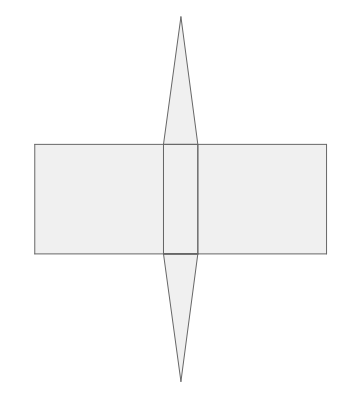
\includegraphics[scale=0.4]{media/es-20/pt217867}
		\task

	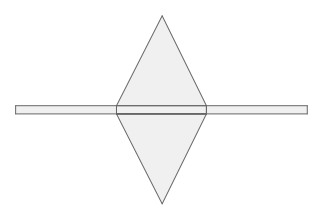
\includegraphics[scale=0.4]{media/es-20/pt555505}
		\task

	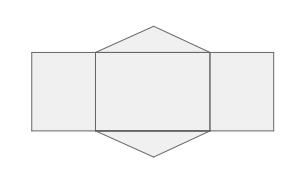
\includegraphics[scale=0.4]{media/es-20/pt701648}
		\task

	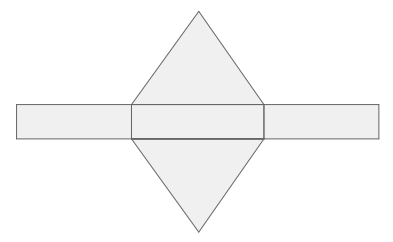
\includegraphics[scale=0.4]{media/es-20/pt815721}
		\task
		
	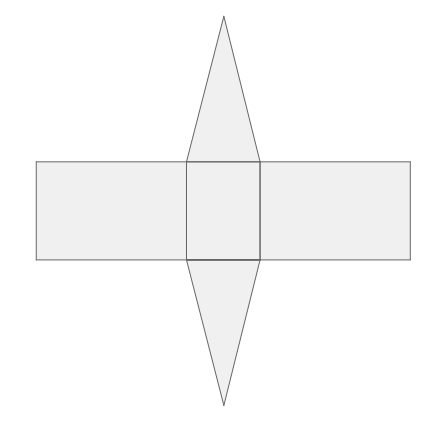
\includegraphics[scale=0.4]{media/es-20/pt458960}
\end{tasks}
\begin{center}
\begingroup
\renewcommand*{\arraystretch}{1.5}
\begin{tabular}{|c|c|c|c|c|c|}
	\hline
&&&&&\\
	\hline
\tikzmath{\t1 = 5.5; \t2 =5.5; \b1=0.5;
% Computations are also possible
\t3 = \t1 *0.5; \p1 =\b1 +3;} 
\begin{tikzpicture}[scale=0.25]
% front face
\coordinate (A) at (0,0);
\coordinate (B) at (\t1,0);
\coordinate (C) at (\t3,\t2);
% vector v defines the leakage angle
\coordinate (v) at (.8,.8);
\draw (A)--(B)--(C)--cycle;
% back face
\coordinate (A') at ($(A)+\b1*(v)$);
\coordinate (B') at ($(B)+\b1*(v)$);
\coordinate (C') at ($(C)+\b1*(v)$);
\draw[dashed] (C')--(A')--(B');
\draw (B')--(C');
\draw[dashed](A)--(A');
\draw(B)--(B');
\draw(C)--(C');
\end{tikzpicture}&
\tikzmath{\t1 = 2.1; \t2 =7.8; \b1=6.7;
% Computations are also possible
\t3 = \t1 *0.5; \p1 =\b1 +3;} 
\begin{tikzpicture}[scale=0.25]
% front face
\coordinate (A) at (0,0);
\coordinate (B) at (\t1,0);
\coordinate (C) at (\t3,\t2);
% vector v defines the leakage angle
\coordinate (v) at (.8,.8);
\draw (A)--(B)--(C)--cycle;
% back face
\coordinate (A') at ($(A)+\b1*(v)$);
\coordinate (B') at ($(B)+\b1*(v)$);
\coordinate (C') at ($(C)+\b1*(v)$);
\draw[dashed] (C')--(A')--(B');
\draw (B')--(C');
\draw[dashed](A)--(A');
\draw(B)--(B');
\draw(C)--(C');
\end{tikzpicture}&
\tikzmath{\t1 = 7; \t2 =1.6; \b1=4.8;
% Computations are also possible
\t3 = \t1 *0.5; \p1 =\b1 +3;}
\begin{tikzpicture}[scale=0.25]
% front face
\coordinate (A) at (0,0);
\coordinate (B) at (\t1,0);
\coordinate (C) at (\t3,\t2);
% vector v defines the leakage angle
\coordinate (v) at (.8,.8);
\draw (A)--(B)--(C)--cycle;
% back face
\coordinate (A') at ($(A)+\b1*(v)$);
\coordinate (B') at ($(B)+\b1*(v)$);
\coordinate (C') at ($(C)+\b1*(v)$);
\draw[dashed] (A')--(B');
\draw (A')--(C');
\draw (B')--(C');
\draw (A)--(A');
\draw (B)--(B');
\draw (C)--(C');
\end{tikzpicture}&
\tikzmath{\t1 = 4.5; \t2 =8.9; \b1=6.0;
% Computations are also possible
\t3 = \t1 *0.5; \p1 =\b1 +3;} 
\begin{tikzpicture}[scale=0.25]
% front face
\coordinate (A) at (0,0);
\coordinate (B) at (\t1,0);
\coordinate (C) at (\t3,\t2);
% vector v defines the leakage angle
\coordinate (v) at (.8,.8);
\draw (A)--(B)--(C)--cycle;
% back face
\coordinate (A') at ($(A)+\b1*(v)$);
\coordinate (B') at ($(B)+\b1*(v)$);
\coordinate (C') at ($(C)+\b1*(v)$);
\draw[dashed] (C')--(A')--(B');
\draw (B')--(C');
\draw[dashed](A)--(A');
\draw(B)--(B');
\draw(C)--(C');
\end{tikzpicture}&
\tikzmath{\t1 = 8.1; \t2 =5.7; \b1=2.1;
% Computations are also possible
\t3 = \t1 *0.5; \p1 =\b1 +3;} 
\begin{tikzpicture}[scale=0.25]
% front face
\coordinate (A) at (0,0);
\coordinate (B) at (\t1,0);
\coordinate (C) at (\t3,\t2);
% vector v defines the leakage angle
\coordinate (v) at (.8,.8);
\draw (A)--(B)--(C)--cycle;
% back face
\coordinate (A') at ($(A)+\b1*(v)$);
\coordinate (B') at ($(B)+\b1*(v)$);
\coordinate (C') at ($(C)+\b1*(v)$);
\draw[dashed] (A')--(B');
\draw (A')--(C');
\draw (B')--(C');
\draw (A)--(A');
\draw (B)--(B');
\draw (C)--(C');
\end{tikzpicture}&
\tikzmath{\t1 = 2.1; \t2 =7.8; \b1=1.9;
% Computations are also possible
\t3 = \t1 *0.5; \p1 =\b1 +3;} 
\begin{tikzpicture}[scale=0.25]
% front face
\coordinate (A) at (0,0);
\coordinate (B) at (\t1,0);
\coordinate (C) at (\t3,\t2);
% vector v defines the leakage angle
\coordinate (v) at (.8,.8);
\draw (A)--(B)--(C)--cycle;
% back face
\coordinate (A') at ($(A)+\b1*(v)$);
\coordinate (B') at ($(B)+\b1*(v)$);
\coordinate (C') at ($(C)+\b1*(v)$);
\draw[dashed] (C')--(A')--(B');
\draw (B')--(C');
\draw[dashed](A)--(A');
\draw(B)--(B');
\draw(C)--(C');
\end{tikzpicture}\\
\hline
\end{tabular}
\endgroup
\end{center}
	}{1}
\end{exop}

\begin{exof}{ES101}{146}{1}
\end{exof}

\begin{exop}{
Associe chaque patron à la perspective cavalière qui lui correspond.

\begin{tasks}(3)
		\task

	\includegraphics[scale=0.3, angle=180]{media/es-20/pdr4-eps-converted-to}
		\task

	\includegraphics[scale=0.3, angle=180]{media/es-20/pdr1-eps-converted-to}
		\task

	\includegraphics[scale=0.3, angle=180]{media/es-20/pdr6-eps-converted-to}
		\task

	\includegraphics[scale=0.3, angle=180]{media/es-20/pdr2-eps-converted-to}
		\task

	\includegraphics[scale=0.3, angle=180]{media/es-20/pdr5-eps-converted-to}
		\task

	\includegraphics[scale=0.3, angle=180]{media/es-20/pdr3-eps-converted-to}
\end{tasks}
\begin{center}
\begingroup
\renewcommand*{\arraystretch}{1.5}
\begin{tabular}{|c|c|c|c|c|c|}
	\hline
&&&&&\\
	\hline
\tikzmath{\t1 = 5; \h2=2; \p3=2;} 
\begin{tikzpicture}[scale=0.25]
% front face
\coordinate (A) at (0,0);
\coordinate (B) at (\t1,0);
\coordinate (C) at (\t1,\h2);
\coordinate (D) at (0,\h2);

% vector v defines the leakage angle
\coordinate (v) at (.8,.8);
\draw (A)--(B)--(C)--(D)--cycle;
% back face
\coordinate (A') at ($(A)+\p3*(v)$);
\coordinate (B') at ($(B)+\p3*(v)$);
\coordinate (C') at ($(C)+\p3*(v)$);
\coordinate (D') at ($(D)+\p3*(v)$);
\draw[dashed] (A)--(A')--(B');
\draw (B')--(C');
\draw[dashed](A')--(D');
\draw(B)--(B');
\draw(C)--(C');
\draw(D')--(C');
\draw(D)--(D');
\end{tikzpicture}&
\tikzmath{\t1 = 6; \h2=4; \p3=3;} 
\begin{tikzpicture}[scale=0.25]
% front face
\coordinate (A) at (0,0);
\coordinate (B) at (\t1,0);
\coordinate (C) at (\t1,\h2);
\coordinate (D) at (0,\h2);

% vector v defines the leakage angle
\coordinate (v) at (.8,.8);
\draw (A)--(B)--(C)--(D)--cycle;
% back face
\coordinate (A') at ($(A)+\p3*(v)$);
\coordinate (B') at ($(B)+\p3*(v)$);
\coordinate (C') at ($(C)+\p3*(v)$);
\coordinate (D') at ($(D)+\p3*(v)$);
\draw[dashed] (A)--(A')--(B');
\draw (B')--(C');
\draw[dashed](A')--(D');
\draw(B)--(B');
\draw(C)--(C');
\draw(D')--(C');
\draw(D)--(D');
\end{tikzpicture}&
\tikzmath{\t1 = 3; \h2=4; \p3=5;} 
\begin{tikzpicture}[scale=0.25]
% front face
\coordinate (A) at (0,0);
\coordinate (B) at (\t1,0);
\coordinate (C) at (\t1,\h2);
\coordinate (D) at (0,\h2);

% vector v defines the leakage angle
\coordinate (v) at (.8,.8);
\draw (A)--(B)--(C)--(D)--cycle;
% back face
\coordinate (A') at ($(A)+\p3*(v)$);
\coordinate (B') at ($(B)+\p3*(v)$);
\coordinate (C') at ($(C)+\p3*(v)$);
\coordinate (D') at ($(D)+\p3*(v)$);
\draw[dashed] (A)--(A')--(B');
\draw (B')--(C');
\draw[dashed](A')--(D');
\draw(B)--(B');
\draw(C)--(C');
\draw(D')--(C');
\draw(D)--(D');
\end{tikzpicture}&
\tikzmath{\t1 = 2; \h2=5; \p3=10;} 
\begin{tikzpicture}[scale=0.25]
% front face
\coordinate (A) at (0,0);
\coordinate (B) at (\t1,0);
\coordinate (C) at (\t1,\h2);
\coordinate (D) at (0,\h2);

% vector v defines the leakage angle
\coordinate (v) at (.8,.8);
\draw (A)--(B)--(C)--(D)--cycle;
% back face
\coordinate (A') at ($(A)+\p3*(v)$);
\coordinate (B') at ($(B)+\p3*(v)$);
\coordinate (C') at ($(C)+\p3*(v)$);
\coordinate (D') at ($(D)+\p3*(v)$);
\draw[dashed] (A)--(A')--(B');
\draw (B')--(C');
\draw[dashed](A')--(D');
\draw(B)--(B');
\draw(C)--(C');
\draw(D')--(C');
\draw(D)--(D');
\end{tikzpicture}&
\tikzmath{\t1 = 2; \h2=2; \p3=3;} 
\begin{tikzpicture}[scale=0.25]
% front face
\coordinate (A) at (0,0);
\coordinate (B) at (\t1,0);
\coordinate (C) at (\t1,\h2);
\coordinate (D) at (0,\h2);

% vector v defines the leakage angle
\coordinate (v) at (.8,.8);
\draw (A)--(B)--(C)--(D)--cycle;
% back face
\coordinate (A') at ($(A)+\p3*(v)$);
\coordinate (B') at ($(B)+\p3*(v)$);
\coordinate (C') at ($(C)+\p3*(v)$);
\coordinate (D') at ($(D)+\p3*(v)$);
\draw[dashed] (A)--(A')--(B');
\draw (B')--(C');
\draw[dashed](A')--(D');
\draw(B)--(B');
\draw(C)--(C');
\draw(D')--(C');
\draw(D)--(D');
\end{tikzpicture}&
\tikzmath{\t1 = 3; \h2=6; \p3=0.5;} 
\begin{tikzpicture}[scale=0.25]
% front face
\coordinate (A) at (0,0);
\coordinate (B) at (\t1,0);
\coordinate (C) at (\t1,\h2);
\coordinate (D) at (0,\h2);

% vector v defines the leakage angle
\coordinate (v) at (.8,.8);
\draw (A)--(B)--(C)--(D)--cycle;
% back face
\coordinate (A') at ($(A)+\p3*(v)$);
\coordinate (B') at ($(B)+\p3*(v)$);
\coordinate (C') at ($(C)+\p3*(v)$);
\coordinate (D') at ($(D)+\p3*(v)$);
\draw[dashed] (A)--(A')--(B');
\draw (B')--(C');
\draw[dashed](A')--(D');
\draw(B)--(B');
\draw(C)--(C');
\draw(D')--(C');
\draw(D)--(D');
\end{tikzpicture}\\
\hline
\end{tabular}
\endgroup
\end{center}
	}{1}
\end{exop}
%
%\begin{exop}{
%	Parmi les figures suivantes, lesquelles sont un patron d'un prisme droit à base triangulaire? Justifie.	
%\begin{multicols}{3}
%	\begin{enumerate}
%		\item
%			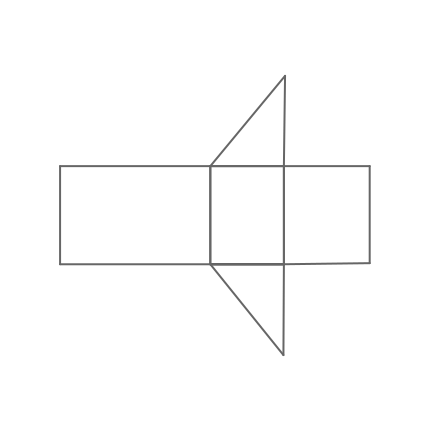
\includegraphics[scale=0.4]{media/es-20/ppd1}
%		\item
%			\includegraphics[scale=0.4]{media/es-20/ppd2}
%		\item
%			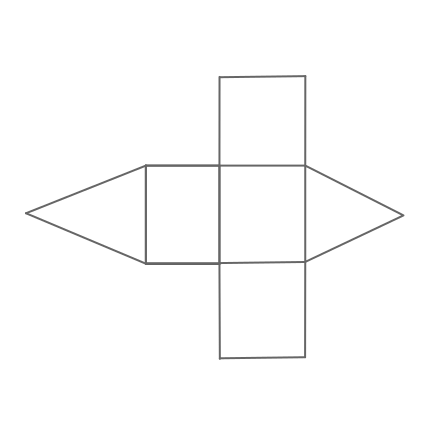
\includegraphics[scale=0.4]{media/es-20/ppd3}
%		\item
%			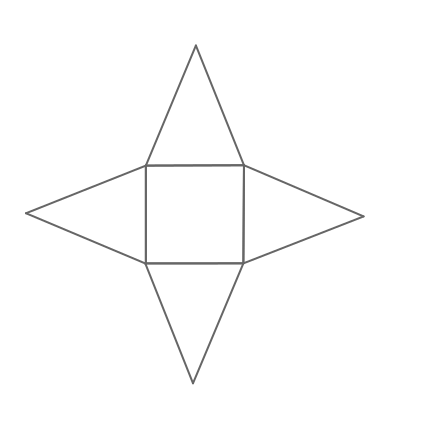
\includegraphics[scale=0.4]{media/es-20/ppd4}
%		\item
%			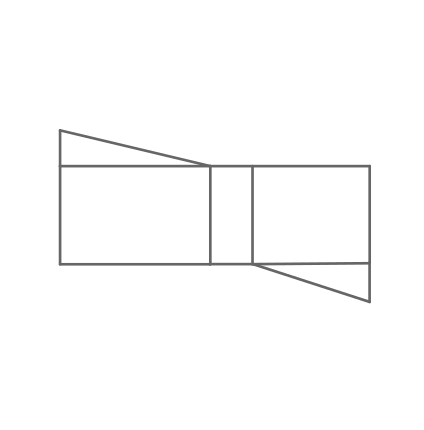
\includegraphics[scale=0.4]{media/es-20/ppd5}
%		\item
%			\includegraphics[scale=0.4]{media/es-20/ppd6}
%	\end{enumerate}
%\end{multicols}
%
%	}{0}
%\end{exop}
\begin{exop}{
Parmi les figures suivantes, lesquelles sont un patron d'un pavé droit? Justifie.	
\begin{tasks}(3)
		\task

			\includegraphics[scale=0.4]{media/es-20/pl1}
		\task

			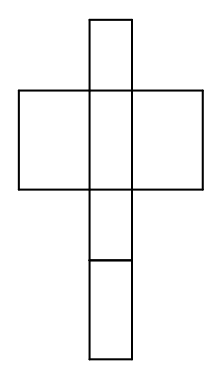
\includegraphics[scale=0.4,angle=90]{media/es-20/pl3}
		\task

			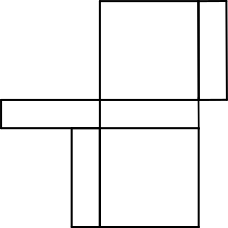
\includegraphics[scale=0.4]{media/es-20/pl5}
		\task

			\includegraphics[scale=0.4,angle=90]{media/es-20/pl6}
		\task

			\includegraphics[scale=0.4]{media/es-20/pl7}
		\task

			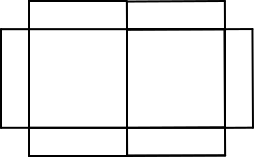
\includegraphics[scale=0.4]{media/es-20/pl8}
\end{tasks}
	}{1}
\end{exop}
\begin{exop}{
	Construit le croquis d'un patron d'un cube de $5cm$ de côté.
	}{1}
\end{exop}

\begin{exop}{
		\begin{minipage}[t]{0.65\textwidth}{
		\vspace{0pt}		
Trace cinq patrons différents d'un dé (en respectant le chiffre indiqué sur chaque face). 
		}
		\end{minipage}
		\hfill
		\begin{minipage}[t]{0.30\textwidth}{
		\vspace{0pt}	
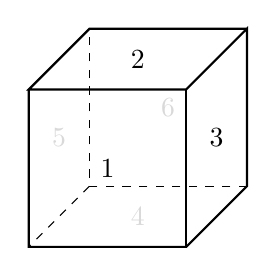
\begin{tikzpicture}
  \draw[thick](2,2,0)--(0,2,0)--(0,2,2)--(2,2,2)--(2,2,0)--(2,0,0)--(2,0,2)--(0,0,2)--(0,2,2);
  \draw[thick](2,2,2)--(2,0,2);
  \draw[dashed](2,0,0)--(0,0,0)--(0,2,0);
  \draw[dashed](0,0,0)--(0,0,2);
  \draw(1,1,2) node{1};
  \draw(1,2,1) node{2};
  \draw(2,1,1) node{3};
  \draw[gray!30](1,0,1) node{4};
  \draw[gray!30](0,1,1) node{5};
  \draw[gray!30](1,1,0) node{6};
\end{tikzpicture}
		}
		\end{minipage}
	}{1}
\end{exop}
\begin{exop}{
		\begin{minipage}[t]{0.65\textwidth}{
		\vspace{0pt}		
Reprends les onze patron de l'exercice 4 et inscrit les chiffre de $1$ à $6$ afin d'en faire les patrons d'un dé (en respectant le chiffre indiqué sur chaque face). 
		}
		\end{minipage}
		\hfill
		\begin{minipage}[t]{0.30\textwidth}{
		\vspace{0pt}	
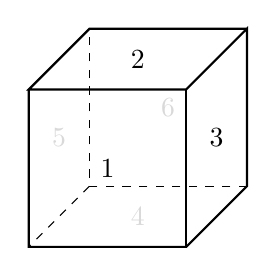
\begin{tikzpicture}
  \draw[thick](2,2,0)--(0,2,0)--(0,2,2)--(2,2,2)--(2,2,0)--(2,0,0)--(2,0,2)--(0,0,2)--(0,2,2);
  \draw[thick](2,2,2)--(2,0,2);
  \draw[dashed](2,0,0)--(0,0,0)--(0,2,0);
  \draw[dashed](0,0,0)--(0,0,2);
  \draw(1,1,2) node{1};
  \draw(1,2,1) node{2};
  \draw(2,1,1) node{3};
  \draw[gray!30](1,0,1) node{4};
  \draw[gray!30](0,1,1) node{5};
  \draw[gray!30](1,1,0) node{6};
\end{tikzpicture}
		}
		\end{minipage}
	}{1}
\end{exop}
\begin{exop}{
Construit le croquis d'un patron d'un parallélépipède rectangle dont:
\begin{tasks}(1)
	\task les côtés de la base mesurent $3cm$ et $7cm$.
	\task La hauteur du prisme mesure $10cm$.
\end{tasks}
	}{1}
\end{exop}
%exercice 8,9,10,14,15,16,17
\begin{exop}{
Construit le croquis d'un patron d'un pavé droit ayant pour dimension $3cm; 6cm$ et $7cm$.
	}{1}
\end{exop}
\begin{exop}{ Ces croquis ont été réalisés rapidement sans faire attention à la longueur des côtés.
	Indique la longueur de tous les segments sur les patrons suivants afin d'obtenir qu'ils correspondent à des patrons de pavés droits.
\begin{tasks}(3)
		\task 	
		
		\includegraphics[scale=0.2, angle=90]{media/es-20/pdm1-eps-converted-to}
		\task 

		\includegraphics[scale=0.2, angle=90]{media/es-20/pdm2-eps-converted-to}
		\task 

		\includegraphics[scale=0.2, angle=90]{media/es-20/pdm3-eps-converted-to}
\end{tasks}

}{1}
\end{exop}
\begin{exop}{ Ces croquis ont été réalisés rapidement sans faire attention à la longueur des côtés.
	Indique la longueur de tous les segments sur les patrons suivants afin d'obtenir qu'ils correspondent à des patrons de pavés droits.
\begin{tasks}(3)
		\task 	

		\includegraphics[scale=0.2, angle=180]{media/es-20/pdm4-eps-converted-to}
		\task

		\includegraphics[scale=0.2, angle=0]{media/es-20/pdm5-eps-converted-to}
		\task 

		\includegraphics[scale=0.2, angle=270]{media/es-20/pdm6-eps-converted-to}
\end{tasks}

}{1}
\end{exop}
\end{document}

